\documentclass[12pt]{beamer}

\usetheme[progressbar=frametitle]{metropolis}
\usepackage{appendixnumberbeamer}

\usepackage[autoplay]{animate}
\usepackage{graphicx}
\usepackage{subcaption}
\usepackage{coloremoji}

\usepackage{booktabs}
\usepackage[scale=2]{ccicons}

%\usepackage{pgfplots}
%\usepgfplotslibrary{dateplot}

\usepackage{xspace}

\newcommand\blfootnote[1]{%
  \begingroup
  \renewcommand\thefootnote{}\footnote{#1}%
  \addtocounter{footnote}{-1}%
  \endgroup
}

\setbeamercolor{normal text}{bg=white}
\newcommand{\themename}{\textbf{\textsc{metropolis}}\xspace}

\title{All the ways you can :$make$ it}
%\subtitle{Running programs from vim}
\date{\today}
\author{Simon Rydell}

% \titlegraphic{\hfill\includegraphics[height=1.5cm]{logo.pdf}}

\begin{document}

\begin{frame}
\titlepage
\end{frame}

%\maketitle
% 
\begin{frame}{Vim in a nutshell}
    \begin{columns}[c]
        \column{4in}
            \begin{figure}[h!]
                \centering
                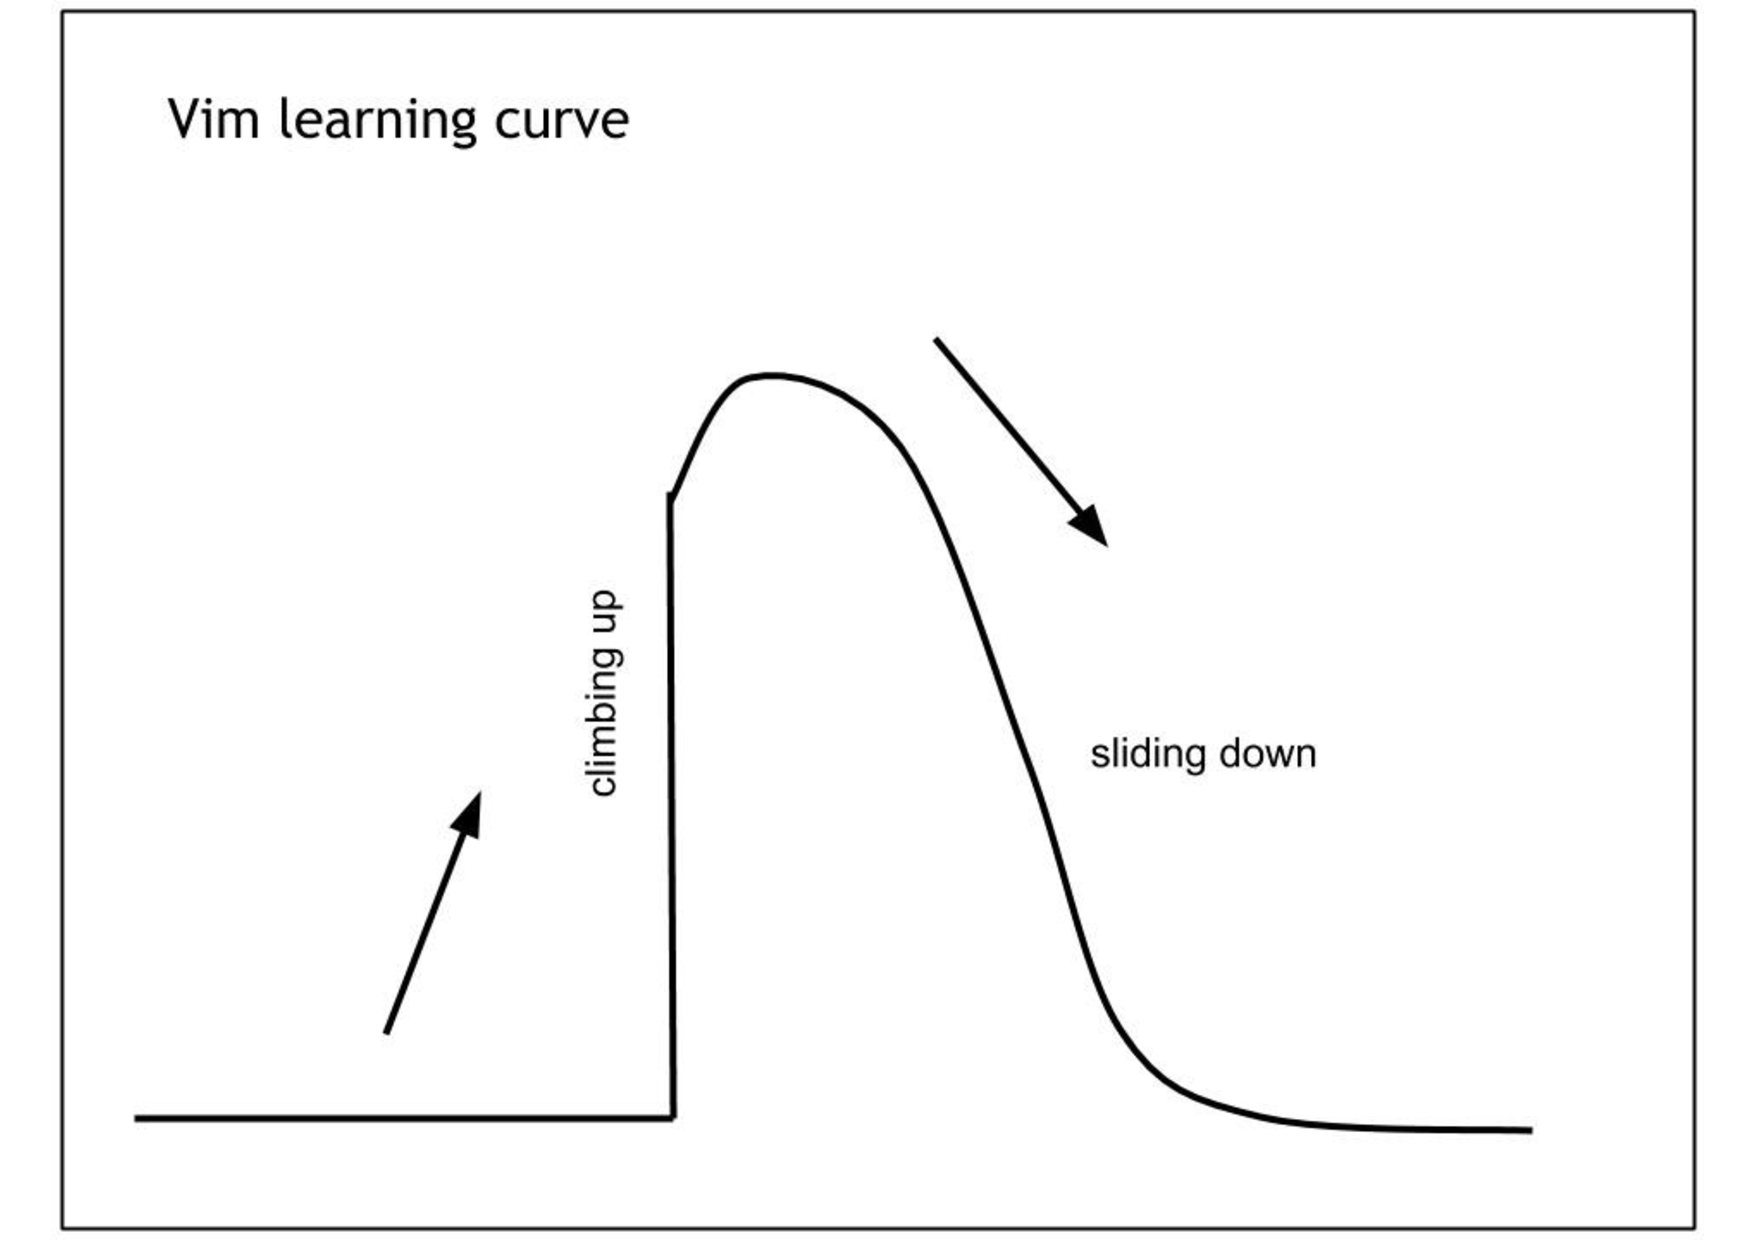
\includegraphics[width=.8\textwidth]{../figures/learingCurve.pdf}
            \end{figure}
    \end{columns}
    \blfootnote{github.com/srydell/tmux-intro}
\end{frame}

% 
\begin{frame}{Overview - Mostly demos}
    \setbeamertemplate{section in toc}[sections numbered]
    \tableofcontents[hideallsubsections]
    \blfootnote{github.com/srydell/tmux-intro}
\end{frame}

% --- Section ---
\section{What about the command line?}

\begin{frame}{What about the command line?}
    \begin{columns}[c]
        \column{4in}
            \Large \textbf{There is no replacing the command line} \\
            \ - Use it from vim
    \end{columns}
    \blfootnote{github.com/srydell/tmux-intro}
\end{frame}

\begin{frame}{How though?}
    \begin{itemize}
        \item :!python3 $\langle$C-R$\rangle\%\langle$CR$\rangle$
        \item vimux
    \end{itemize}
    \blfootnote{github.com/srydell/tmux-intro}
\end{frame}

% --- Section ---
\section{:$make$ steals the show}

\begin{frame}{:$make$ steals the show}
    \begin{itemize}
        \item The native way to build and run scripts from within vim
        \item errorformat
        \item quickfix list
        \item :compiler
    \end{itemize}
    \blfootnote{github.com/srydell/tmux-intro}
\end{frame}

% --- Section ---
\section{Dispatch the saviour}

\begin{frame}{Dispatch the saviour - tpope}
     \begin{itemize}
         \item vim-dispatch
         \begin{itemize}
             \item Asynchronous :$make$ with :$Make$
             \item Sending build processes to other windows (e.g. tmux panes)
         \end{itemize}
         \item vim-projectionist
         \begin{itemize}
             \item Stores metadata about your project
             \item Glob specific $makeprg$
         \end{itemize}
     \end{itemize}
     \blfootnote{github.com/srydell/tmux-intro}
\end{frame}

\begin{frame}{Questions?}
     \begin{center}
         \large :set makeprg=echo\textbackslash \ Questions\textbackslash?\\
         \LARGE :make
     \end{center}
     \blfootnote{github.com/srydell/tmux-intro}
\end{frame}


\end{document}